\section{Remote Server}
\label{sec:test-rs}

In the Remote Server application, the tests that were needed to make were exclusively with the good creation of the database, the connection between local system and remote client and the upload and update local system.

In Fig.~\ref{fig:rs-db-test} is the proof that the database was well created with the scripts created.
%
\begin{figure}[!htb]
    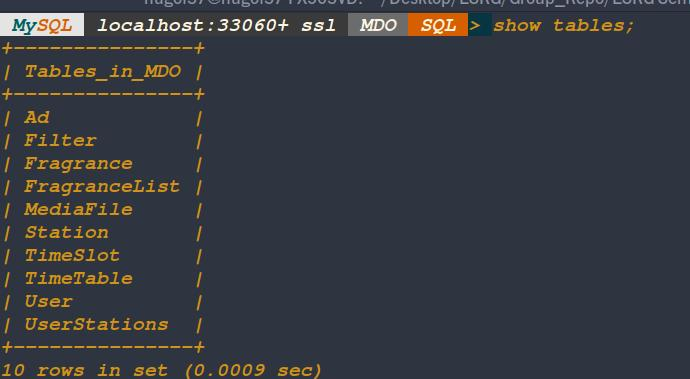
\includegraphics[width=.5\textwidth]{img/rs-db-test.jpg}%
  \caption{Database Test Case}%
  \label{fig:rs-db-test}
\end{figure}

Now, on Figure~\ref{fig:rs-server-test} is a validation of the connection between local system and remote client.
%
\begin{figure}[!htb]
    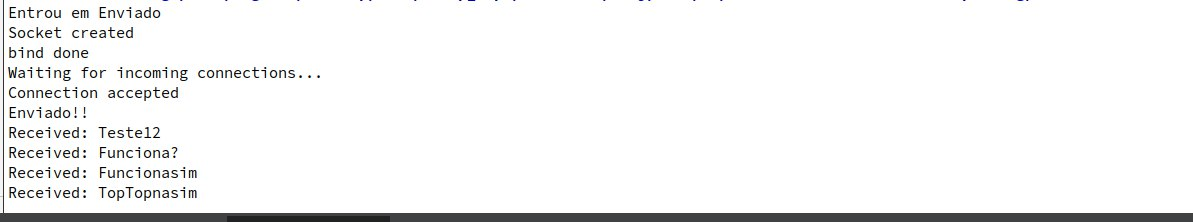
\includegraphics[width=.7\textwidth]{img/rs-ls-test.jpg}%
  \caption{Communication Between systems Test Case}%
  \label{fig:rs-server-test}
\end{figure}

Lastly, on Fig.~\ref{fig:rs-upload-test} and Fig.~\ref{fig:rs-download-test} is the Test case of the update of the local system uploading the file of a new Ad.
%
\begin{figure}[htb!]
  \centering
  \begin{subfigure}{.7\textwidth}
    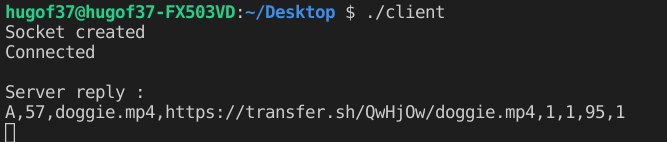
\includegraphics[width=\textwidth]{img/rs-upload-test.jpg}%
  \caption{Send and upload of file}%
  \label{fig:rs-upload-test}
  \end{subfigure}
  % 
  \begin{subfigure}{.6\textwidth}
    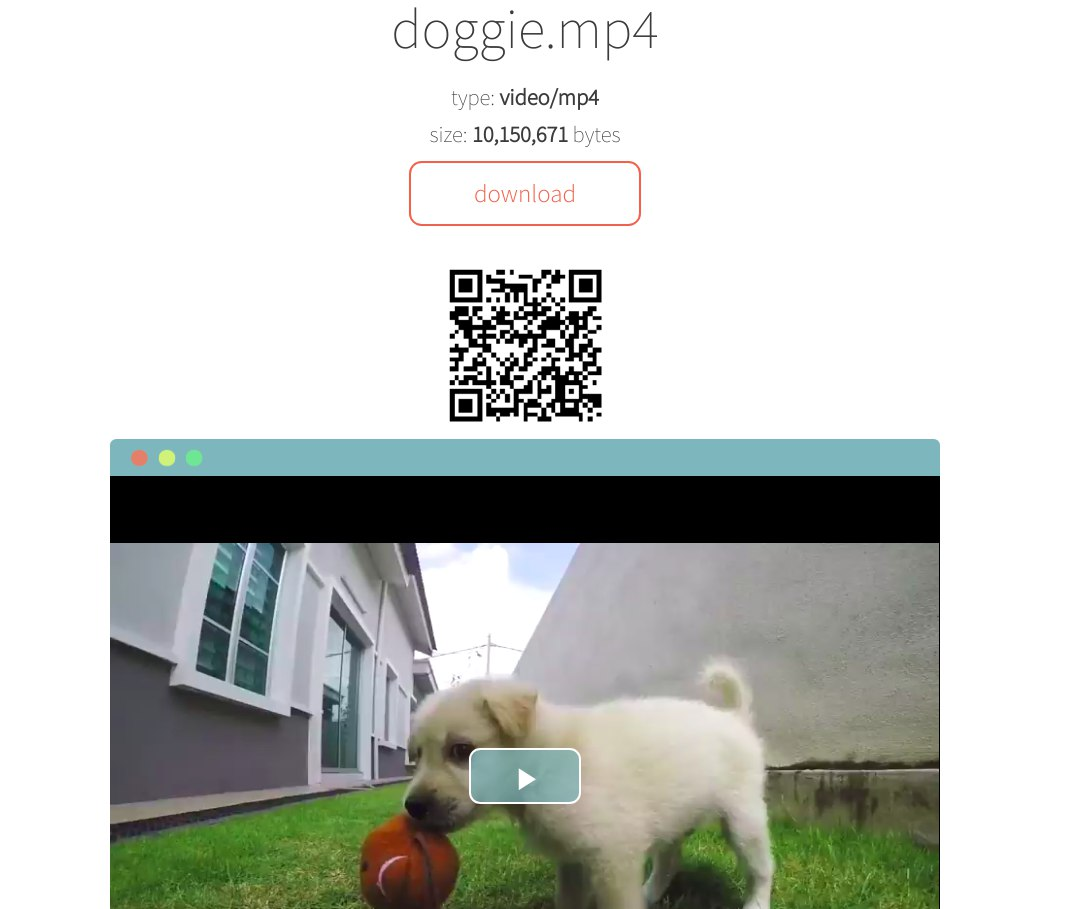
\includegraphics[width=\textwidth]{img/rs-download-test.jpg}%
  \caption{Download of file}%
  \label{fig:rs-download-test}
  \end{subfigure}
  % 
  \caption{Update and upload Test}%
  \label{fig:rs-update-upload-test}
\end{figure}